Through the earlier experimentations with the graph generations based on specific properties, improvements have been made. This includes normalisation of the values into the range of 0-10 rather than using a scale factor. Which ensures that all the graphs will be similarly shaped and have the same axis size for an easier visual comparison. Also I've included page rank as well as the other graph properties used before. Finally the datasets I will use will be generated through my program by an input of text. Afterwards will be converted into graphs where the words represent the vertices and the edges are directed to the next word in the order of the text. A factor that affected the dataset was the punctuation so to achieve congruent data, the punctuation are stripped unless they are sentence enders such as full stops, question marks, exclamation marks etc. 

Therefore, the graph we experiment on are directed graphs generated from various language families.

\section{Linguistics}
Modern languages are descendants of ancestral languages through evolution of linguistics. Through the different ages of the world, language has always been a key part in communication between societies. They are developed and taught to newer generations to reach the stages in the current world. The history of languages can be viewed as a family tree where modern languages are nearer the bottom. Along this trees, there are groups of languages that share a common ancestor. These are the \emph{language family} of those languages.

Estimations of around 500 language families exist and Campbell \cite{campbell2018many} has reported that there are exactly 406 independent language families including dead languages and \emph{language isolates} (where the language does not fit into a language family). According to Ethnologue\cite{eberhard2023a}, who are the research centre for language intelligence, there are 142 different living language families. Of the living families, six are considered to be the major families and are Indo-European, Afro-Asioatic, Niger-Congo, Austronesian, Sino-Tibetan and Trans-New Guinea.

The aim of my research is to study modern languages that fall under the Indo-European language family and the Sino-Tibetan language family. The main families are known as the \emph{proto-language} as they are the parent language where many languages are derived from\cite{rowe2022concise}. The languages being English, German and Dutch that are Germanic language under the Indo-European family. Russian and Polish which are Balto-Slavic language under Indo-European family.  French and Spanish which are Latin languages under the Indo-European language. Finally Chinese which falls under the Sino-Tibetan family. Furthermore, I will also look at Japanese which part of the Japonic language family but it would be considered a language isolate if the Ryūkyūan languages were not distinct from Japanese\cite{campbell2010language}. Therefore these are all the languages in which I will translate the text extract into datasets.

\section{Text Corpus}
The best way in comparing the results to other languages is to have a dataset that is based on the same text extract. Thus, the text extract that is chosen should be simple and well know, in my case, I have chosen to use the popular story in all languages, "Sleeping Beauty". To ensure that the same version is used, the Grimm Brothers version is utilised where the original was in German and extracted from the book of children stories "Kinder- und Hausmärchen"\cite{grimm1857kinder}. So using translations of this story, graphs are generated based on each language studied.  Additionally, instead of using the entirety of the story, the first two paragraphs are used so that the graphs are not overwhelmingly dense which tells the story as follows:
\begin{quote}
In times past there lived a king and queen, who said to each other every day of their lives, "Would that we had a child!" and yet they had none. \dots There were thirteen of them in his kingdom, but as he had only provided twelve golden plates for them to eat from, one of them had to be left out.
\end{quote}
In conclusion the original nine dataset created in this way can be used for graph property calculations. Next section will study English version of the story which is part of the I

\section{Indo-European Language Family}
Initial the languages of the Indo-European family are studied and a few of them are described in detail later including English and German. Throughout the analysis, words are referred to as vertices, the two paragraph extract of "Sleeping Beauty" in the relative language will be referred as the story corpus and vice versa. Each word in a graph has edges which are directed to the next word relative to the two paragraph extract. 
\subsection{English}
English words can be organised into eight different parts of speech; Nouns, Pronouns, Adjectives, Adverbs, Verbs, Prepositions, Determiners and Conjunctions. Linguistic researchers focus on the use of these categories in different situations such as through speaking or through magazines\cite{khaisaeng2017study}. We will study the appearances of these categories in our story corpus. To achieve this, the story corpus is received as an input to my program so it may generate a usable dataset. The dataset is then converted into a directed word graph as shown by figure \ref{fig:engword}. Additionally in replacement of having each vertex labelled by the corresponding word, each vertex will be labelled with an integer. The relative integer for each word will be shown on the table of values for the graph. The table will be shown later in Table \ref{table:english}. So we achieve the initial directed word graph both in original form and alternated form shown in figure \ref{fig:engnum}.

\begin{figure}[H]
\centering
\begin{subfigure}{.45\textwidth}
	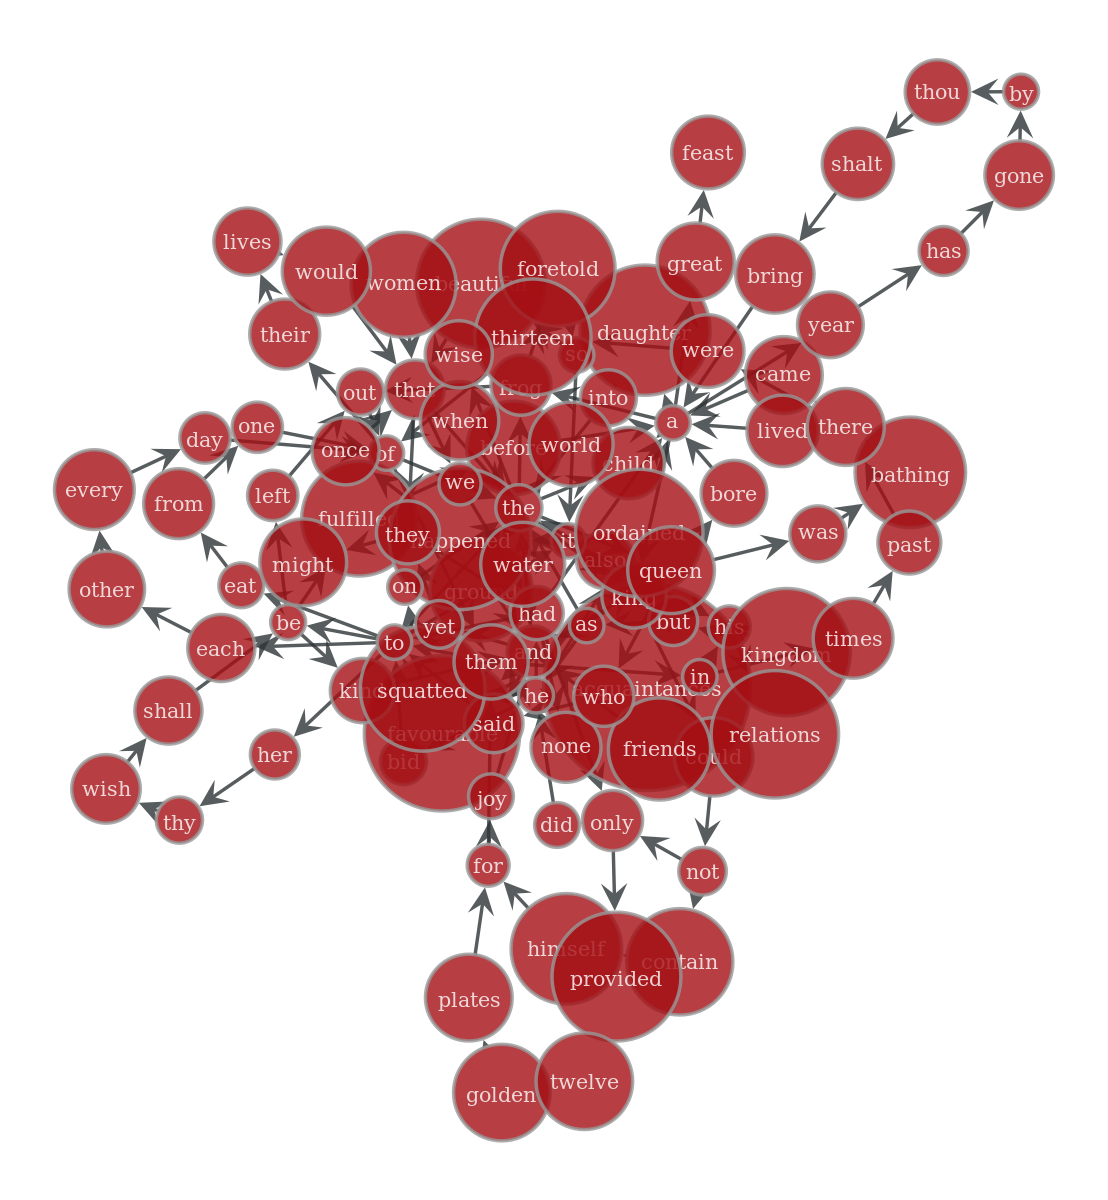
\includegraphics[scale=0.2]{englishwordgraph.png}
	\caption{Graph generated based on an extract of the story "Sleeping Beauty" with each unique word labelling each vertex.}
	\label{fig:engword}
\end{subfigure}
\hfill
\begin{subfigure}{.45\textwidth}
	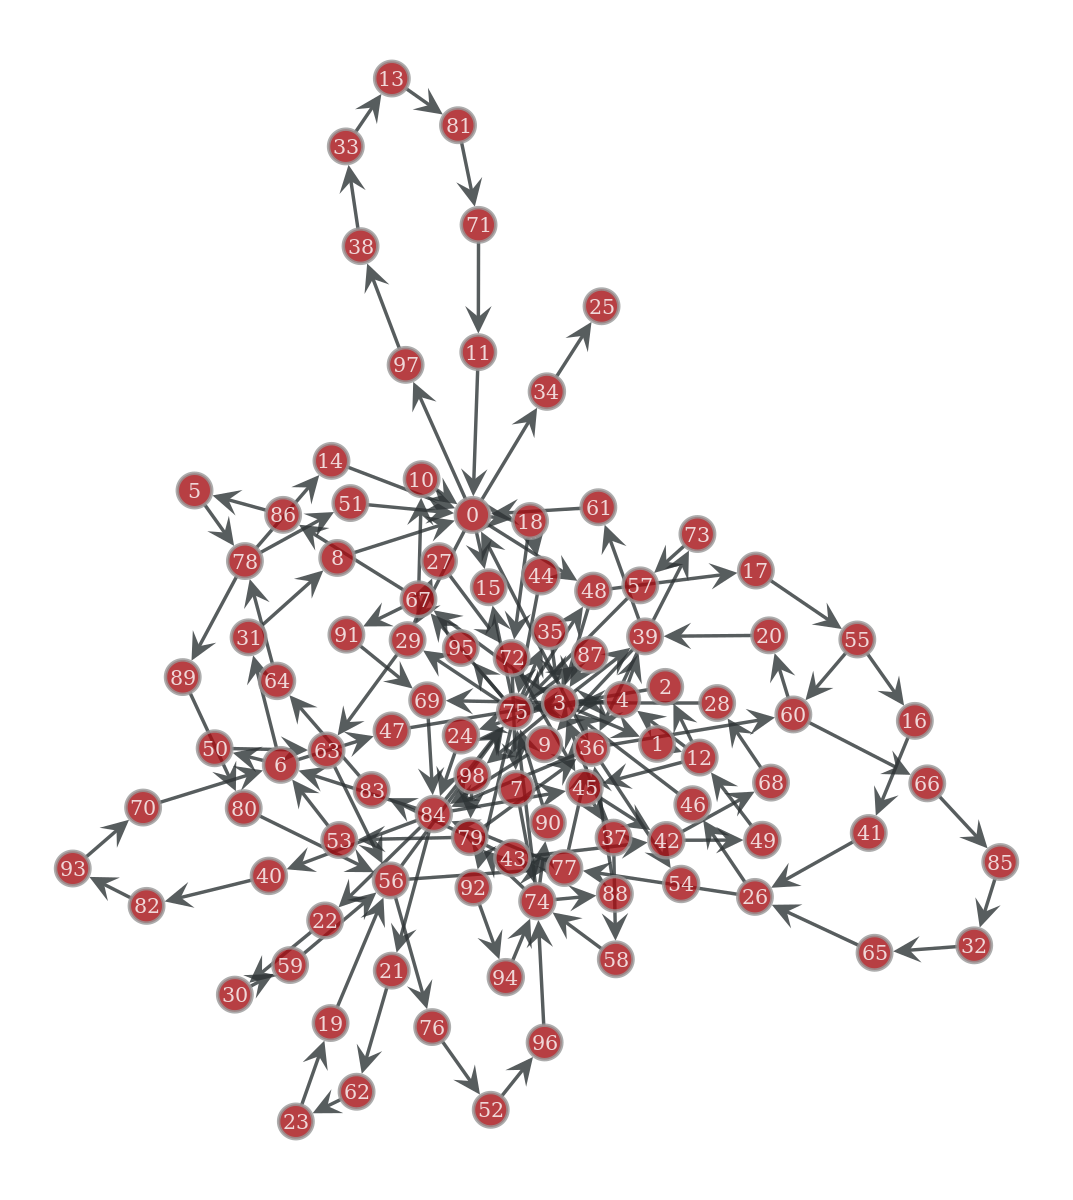
\includegraphics[scale=0.2]{englishnumbergraph.png}
	\caption{Same graph as the word graph for the English version of "Sleeping Beauty" but with numerical labelling rather than the corresponding words. The numbers are labelled in order of the unique words in alphabetical order which is also shown in the table later on.}
	\label{fig:engnum}
\end{subfigure}
\caption{Graph created from the corpus labelled with words or in integers.}
\end{figure}

As done in the Early Experimentations of the karate club dataset, we calculate the values of the various graph properties explained in Chapter 2. These are graph properties such as local clustering coefficient, betweenness centrality, closeness centrality, trophic levels and page rank. Values are organised into their corresponding columns and presented as a table with the ten most frequent words shown in Table \ref{table:englishtop} below. Table also includes the number of appearances the word has denoted as count and the relative vertex number in the numbered English graph. The entire table can be seen in Appendix \ref{app:engtable}.

\begin{table}[H]
\centering
\begin{subtable}{.45\textwidth}
	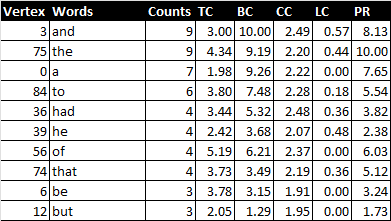
\includegraphics[scale=0.9]{englishtabletop10.png}
	\caption{The first 10 most common words of the dataset. Generated from the English version of "Sleeping Beauty" in a table format. }
	\label{table:englishtop}
\end{subtable}
\hfill
\begin{subtable}{.45\textwidth}
	\hspace{1.5cm} 
	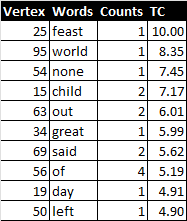
\includegraphics[scale=1]{engtabletc.png}
	\caption{Top 10 words ranked by their trophic levels based on the English Story Corpus.}
	\label{table:englishtoptc}
\end{subtable}
\caption{Partial extracts of the table data for graphical properties of the English Story Corpus.}
\end{table}

We begin by analysing words with the most recurrences which are, in the order of most frequent to least, "and", "the", "a", "to", "had", "he", "of", "that", "be" and "but". Note that nouns, adverbs and adjectives do not appear in the most recurring words. These are the words that are deemed more vital in the creation of structure within a sentence. Any sentence in "Sleeping Beauty" will have a high chance of containing at least one of these words. Since this is a small dataset, we can compare these words to a larger dataset for word reoccurrences as the Zipf curve for language are similar as discussed in a previous section. We choose to compare the story corpus to the British National Corpus (BNC)\cite{bnc2007british} which is a 100 million word collections that includes both written and spoken language. The benefits in choosing BNC is that it contains older English so may provide clearer correlations to the story of "Sleeping Beauty" as the Brothers Grimm version began in the late 18th century. Hence for the BNC, the top ten frequent words\cite{leech2014word} in order of frequency are; "the", "of", "and", "a", "in", "to", "it", "is", "to" and "was". Comparing the most frequent words in both corpuses, correlations are achieved such as the repetitions of words "the", "to" etc. Such similarities reinforce the fact that the English language has a structured form that requires the use of these such words, as demonstrated with a much smaller corpus compared to the the BNC.

Now onto the analysis of Trophic levels and coherence (see Table \ref{table:englishtoptc}). When applying trophic level calculations on directed word graphs, the levels represent the position of the word in a sentence similarly shown in the analysis of network data in empirically-derived directed networks\cite{johnson2017looplessness}. For the "Sleeping Beauty" English word graph, the lower trophic levels tends to be sentence starters and the higher levels are the ends of sentences. This is supported by the data because the top five words with largest trophic levels values (ranging from 10.00-6.01) are all sentence enders. Along with the bottom five being words (trophic values ranging from 0.49-0.00) nearer the start of sentences such as "there" and "times" in relation to the corpus. However trophic incoherence is calculated to be 0.969 which means that the levels in the graph can not be distinguished and are not clear. Since the $\text{trophic coherence} = 1 - \text{trophic incoherence} = 0.03$ which is due to the fact of the vast difference of sentence lengths in the corpus. Which varies from the shortest sentence of five words and the longest of forty seven words. Consequently the for the extract used, it may not provide a clear hierarchical layout but still provides a good layout of sentence flow from the lowest level to the highest level. Demonstrated by further graphs with the trophic levels as the y-axis ranging from 0 at the top to 10 at the bottom to provide a normal cascade of words. Includes other graphical properties starting with betweenness and closeness centrality (Figures \ref{fig:engbc} and \ref{fig:engcc}) shown next.

\begin{figure}[H]
\centering
\begin{subfigure}{.45\textwidth}
	\hspace{-1cm} 
	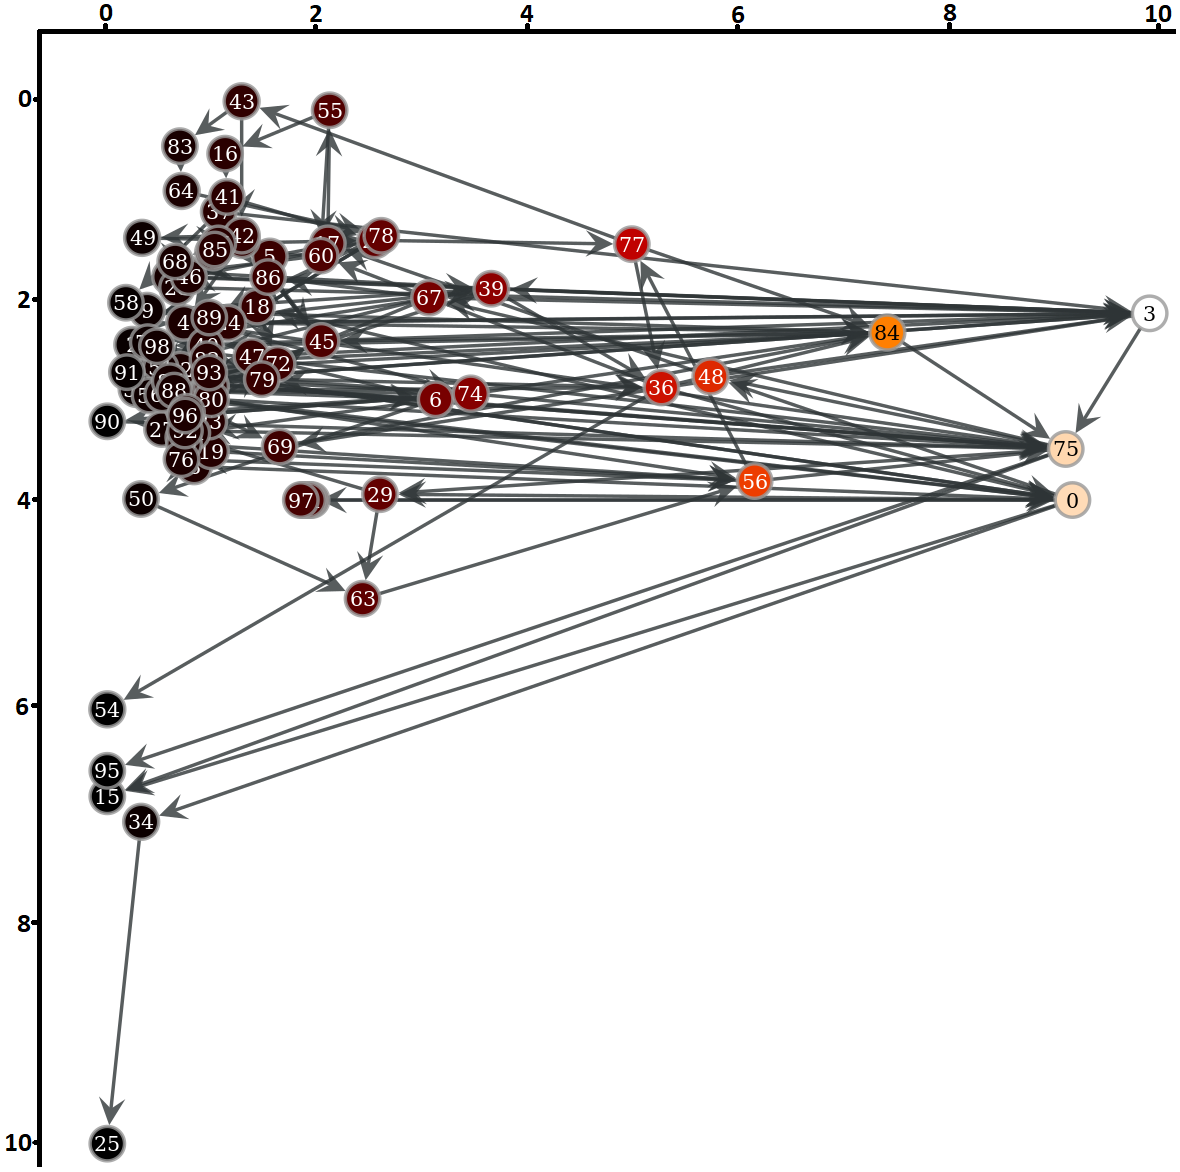
\includegraphics[scale=0.2]{englishbetweenness.png}
	\caption{Numbered English graph positioned with trophic levels (y-axis) against the betweenness centrality (x-axis).}
	\label{fig:engbc}
\end{subfigure}
\hfill
\begin{subfigure}{.45\textwidth}
	\hspace{-1cm} 
	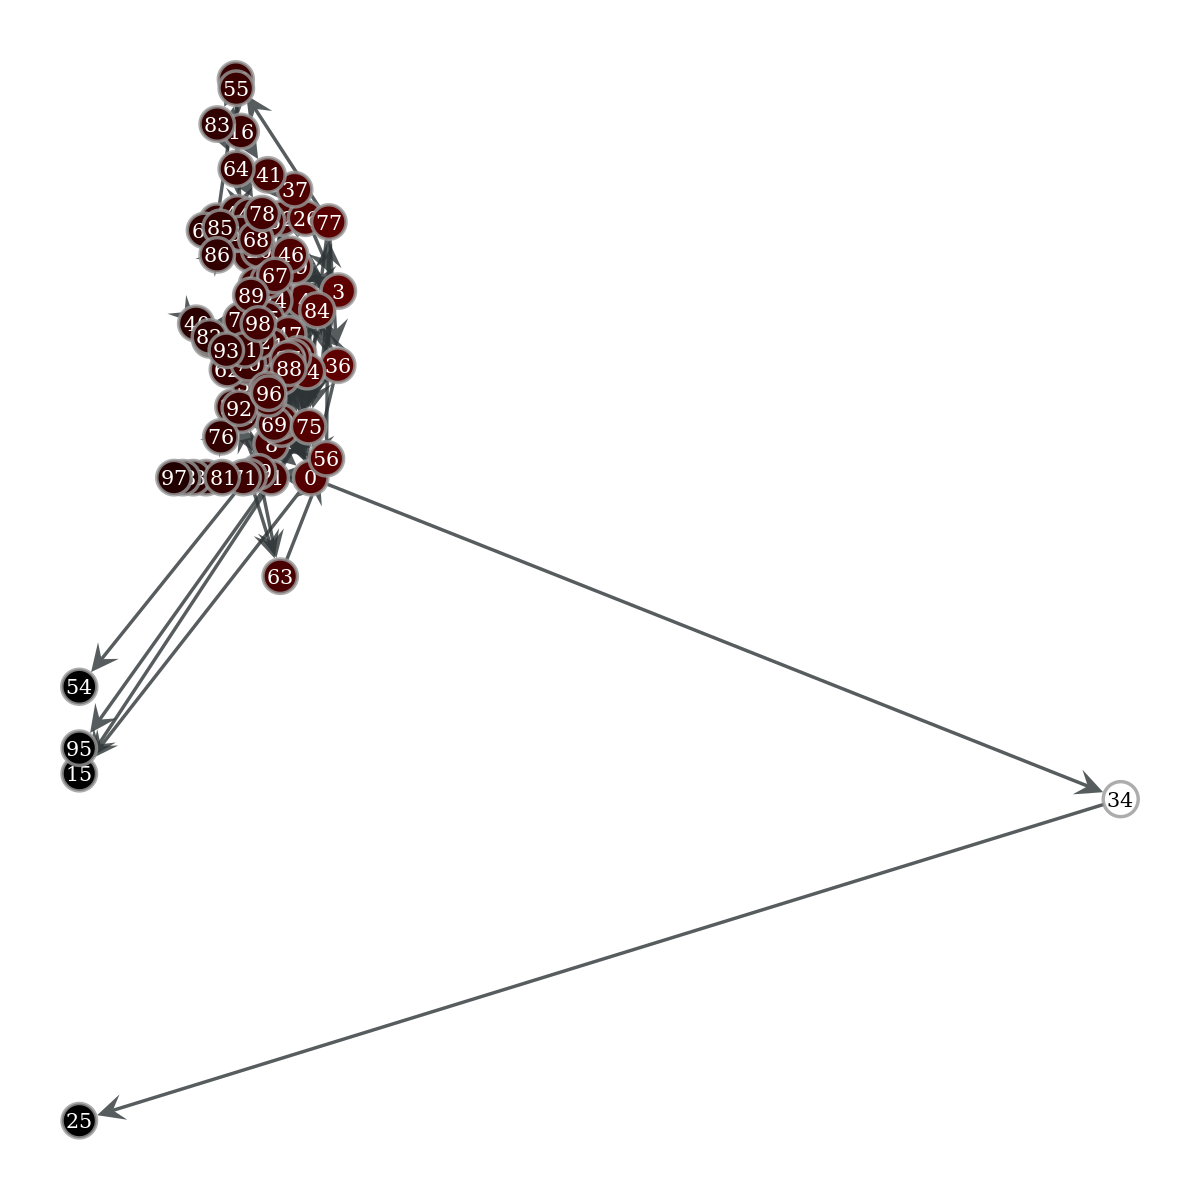
\includegraphics[scale=0.2]{englishcloseness.png}
	\caption{Numbered English graph positioned with trophic levels (y-axis) against the closeness centrality (x-axis).}
	\label{fig:engcc}
\end{subfigure}
\caption{Betweenness and closeness centrality values displayed on the x-axis in graphical form.}
\end{figure}

As visually demonstrated on Figures \ref{fig:engbc} and \ref{fig:engcc}, the centrality values for each word is plotted against their trophic levels. Both have been normalised to a range of 0-10 with Figure \ref{fig:engbc} showing the betweenness centrality on the x-axis and Figure \ref{fig:engcc} showing the closeness centrality. Key vertices identified in relation to their betweenness values are vertex 3, 0 and 75 which are the words "and", "a" and "the" respectively. These are conjunctions and determiners of the English language and they have the largest frequency of appearance in the corpus relating to the word counts discussed before. So, there is a strong link between the betweenness centrality of vertices to the word counts in the text. Furthermore, these words are common in forming correct structure of an English sentence meaning that high betweenness associates the words as key bridges within a sentence. 

When considering closeness centrality, the graph shows that almost all vertices have a larger closeness value in comparison to their betweenness. This is because the closeness analyses the importance of the words as within their clusters rather than the graph as a whole. So words with high closeness are key connectives in their relative clusters, in other words the sentences they are part of. However vertex 34 (the word "great") is an outlier and by further analysis, vertex 34 is the only connect between vertex 0 and 25. Vertex 25 having the highest trophic level and vertex 0 has a low trophic level and a higher degree. Consequently, the closeness value for 34 is much higher due to the fact that it is the only predecessor of vertex 34 which in itself only has one predecessor. Thus meaning that vertex 34 is the only local bridge in it's sentence giving it an extreme closeness.

In conclusion, based on the story corpus, betweenness finds the words most commonly used as connectors in sentences given the whole extract and closeness finds the words as connections within a close range of one another.

\begin{figure}[H]
\centering
\begin{subfigure}{.45\textwidth}
	\hspace{-1cm} 
	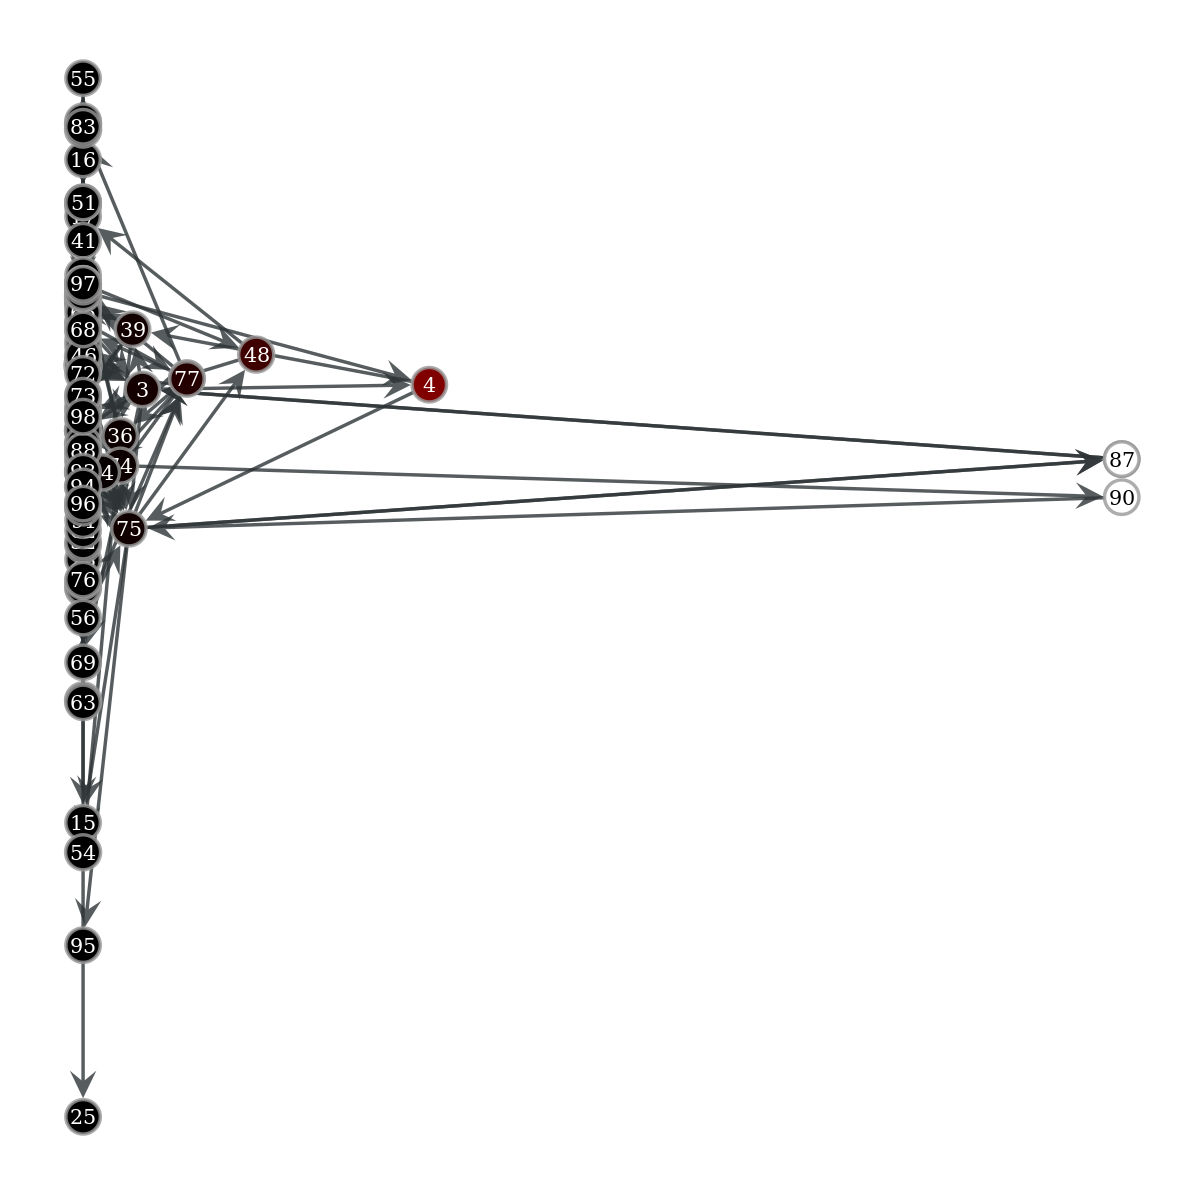
\includegraphics[scale=0.2]{englishlocalclustering.png}
	\caption{Numbered English graph positioned with trophic levels (y-axis) against the local clustering coefficient (x-axis).}
	\label{fig:englc}
\end{subfigure}
\hfill
\begin{subfigure}{.45\textwidth}
	\hspace{-1cm} 
	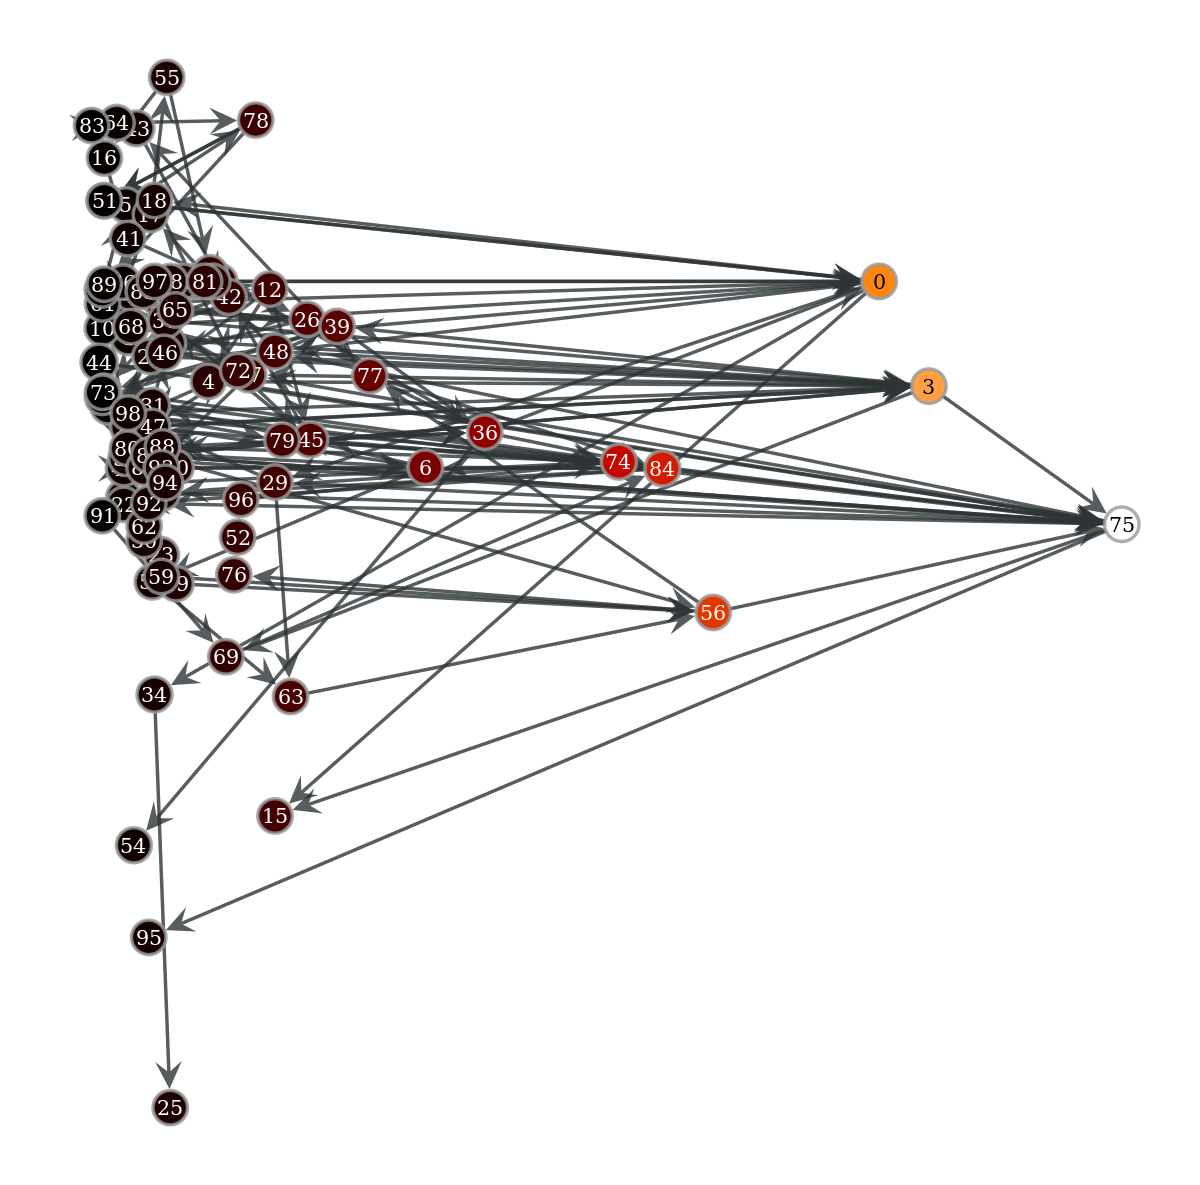
\includegraphics[scale=0.2]{englishpagerank.png}
	\caption{Numbered English graph positioned with trophic levels (y-axis) against the page rank (x-axis).}
	\label{fig:engpr}
\end{subfigure}
\caption{Similarly as before with betweenness and closeness but with local clustering and page rank instead.}
\end{figure}

Finally Local Clustering and Page rank of the vertices in the graph are presented similarly as before with it's local clustering in Figure \ref{fig:englc} and page rank as Figure \ref{fig:engpr}. Immediately, the local clustering graph shows very few vertices who has a high local clustering, the main ones being vertices 87 and 90 (words "water" and "when" respectively). However, these do no give a clear relation other than the words connected to and from these vertices have a high degree or importance in the graph. These are words such as "and" and "a". On the other hand this is only for the English version of the story so other languages may lead to different results. The page rank of each vertex shows the importance of each word beyond their direct contact. Essentially it has elements of both closeness and betweenness centrality which the graph reinforces.

In conclusion, when analysing the English language, trophic levels have provided a naturally flow of data presentation from top to bottom in the various graphs generated. Some sections are of the graph are also grammatically correct. Betweenness Centrality and Page rank both identifies the words of most importance with respects to the words that connect them. Closeness centrality also identifies words of key importance but at a local level. As this is a smaller corpus, these words are similar. Finally the Local Clustering does not provide sufficient benefit when visualising the dataset in the English language. Therefore the results generated based on the English version can be expanded to represent the English language and can even be used to predict and analyse unknown texts or missing words with a given text by representing the missing words as vertices. The position of the vertices will determine it's importance and use within a sentence. This is of course for the English language or language with similar structure.

Now we move onto the analyse of a different translation of the corpus, German.

\subsection{German}
German is a Germanic language under the Indo-European language family, same as English. However whilst Modern English no longer use inflectional case system, the German language still does\cite{durrell2011hammer}. So as well as the parts of speech like in English, German words can be divided into two groups, the ones who are \emph{inflectable} and \emph{uninflectable}. If a word is inflectable then their form changes based on the context that the word is used in. These include the three genders for the words, the four cases (nominative, accusative, genitive and dative) and number (singular or plural). Uninflectable words are known as modal particles and mainly used to highlight an emotion of the sentence in spoken language. Therefore German language considerably more varied than the English language so the dataset in theory would contain more unique words overall. This is proven to be true as the dataset for German contains 109 words whilst English had 99.

Expectations of the graph properties for the German language is that there would be more unique words of higher importance based on the different genders for words. On average, sentence lengths should also be longer due to the generated words which will be seen in trophic levels if it is the case. Word graphs for the German version of the corpus are generated and shown in figure \ref{fig:gergraph}. Similarly as before, each number references the same word in it's position.

\begin{figure}[H]
\centering
\begin{subfigure}{.45\textwidth}
	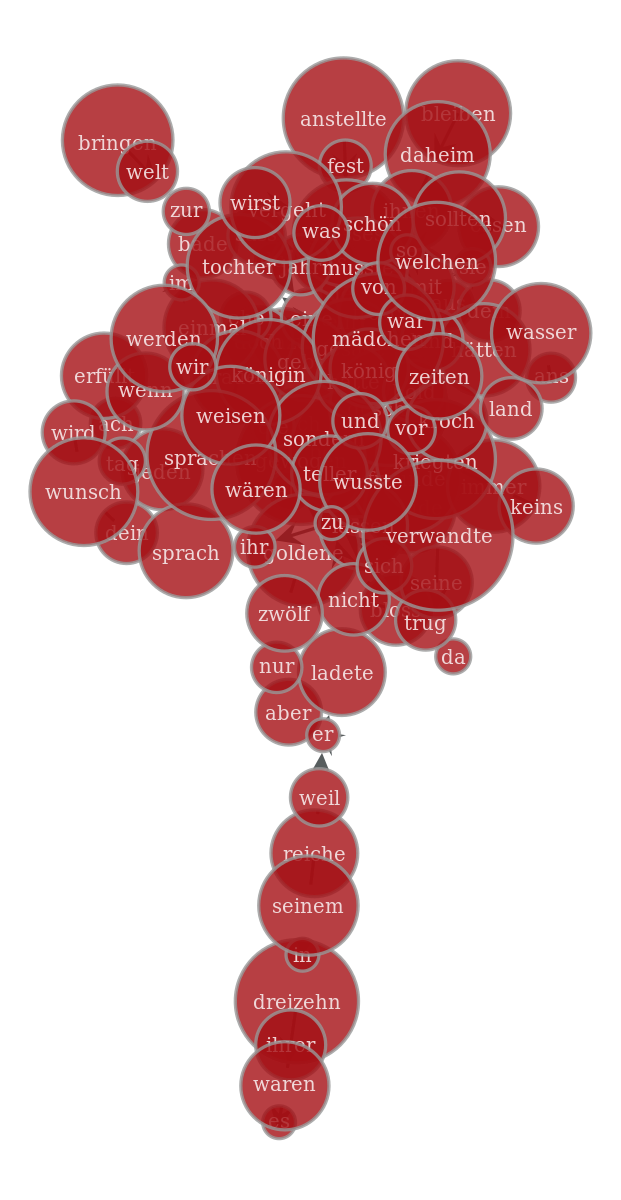
\includegraphics[scale=0.2]{germanwordgraph.png}
	\caption{German word graph generated based on the German translation of the corpus.}
	\label{fig:gerword}
\end{subfigure}
\hfill
\begin{subfigure}{.45\textwidth}
	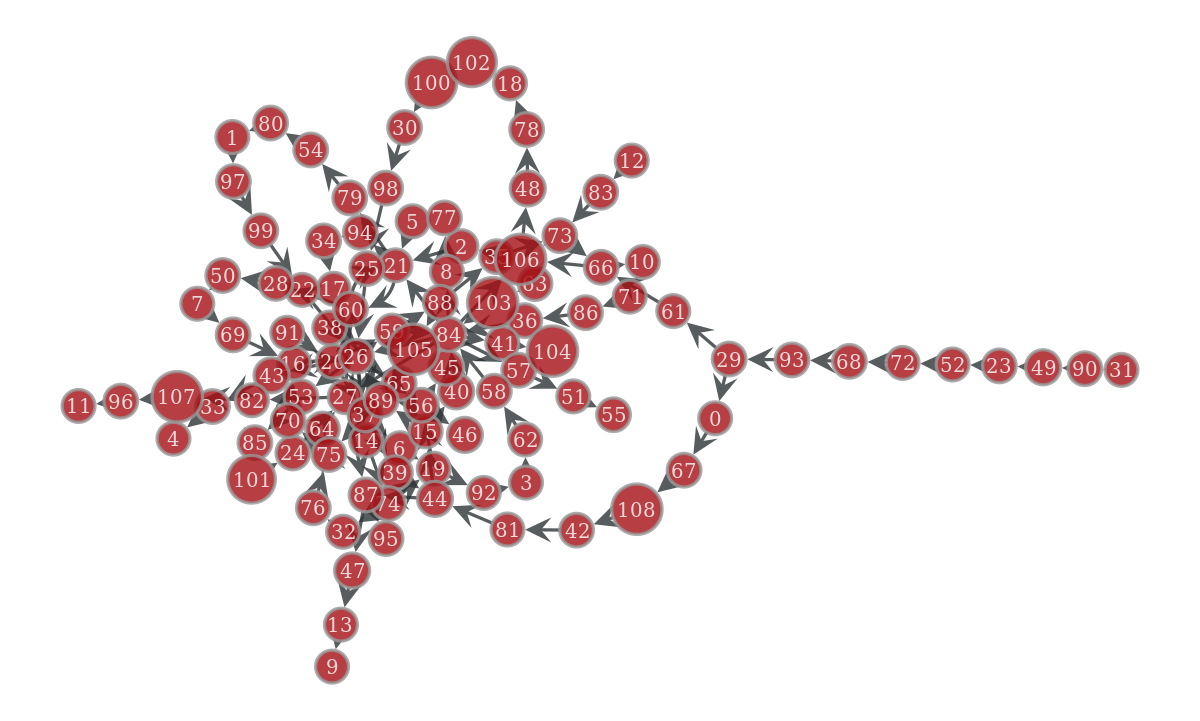
\includegraphics[scale=0.2]{germanwordgraphnumbered.png}
	\caption{Numbered version of the word graph to provide a clearer graph. This is called the German numbered graph.}
	\label{fig:gernum}
\end{subfigure}
\caption{The German word graph and numbered equivalent of the word graph generated from the German translation of the "Sleeping Beauty" corpus.}
\label{fig:gergraph}
\end{figure}

Table \ref{table:germantop} shows the most common ten words in the German dataset along with each graph property value. The translation to English for each word in the order of the table is as follows; "and", "a" (Masculine), "the" (Feminine), "to", "a" (Feminine), "Queen", "King", "not", "himself/herself/itself" (dependent on the pronoun this refers to) and "the" (Neutral). As expected when comparing to the English dataset most words appear in both translations as the top ten, in particular the top three. Which we recall was "and", "the" and "a". However rather than a cumulative count of "the" in English, the German translation has multiple versions which may counteract each others importance. By retaining the inflectable changes, the average count is lower for the German translation. Additionally the range has also decreased. For example, "the" in English was split into "die", "der" and "das" in German. By noting these key differences, the graphical properties will be analysed starting with trophic coherence.

\begin{table}[H]
\centering
\begin{subtable}{.45\textwidth}
	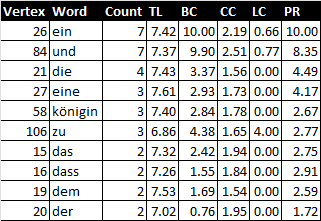
\includegraphics[scale=0.9]{germantabletop10.png}
	\caption{Top 10 words with the highest frequency in the German translation of the corpus. Shown in table format with other graphical properties. }
	\label{table:germantop}
\end{subtable}
\hfill
\begin{subtable}{.45\textwidth}
	\hspace{1.5cm} 
	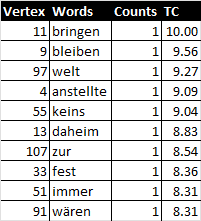
\includegraphics[scale=1]{gertabletc.png}
	\caption{Top 10 works with highest trophic levels in the German translation dataset.}
	\label{table:germantoptc}
\end{subtable}
\caption{Partial extracts of the table data for graphical properties of the German Story Corpus.}
\end{table}

Analysing the trophic levels, top ten seen in Table \ref{table:germantoptc}, the results show that most words congregate at around 7.1. This can be more evidently seen in visual representations on figures \ref{fig:gercentrality} and \ref{fig:gerother}. From the same figures, there is a unique path from vertex 31 to 29 which is equivalent "Es waren ihrer dreizehn in seinem Reiche, weil er". This is the beginning of a sentence belonging to the German story corpus and holds all unique words that are not used in other sentences. Hence has not been influenced by other vertices so has a clear hierarchical structure which leads to the low trophic levels. Whereas most other sentences share words which causes the conglomeration nearer 7. So the German language has more options for word choices that causes the increased possibility of unique sentences. Meaning that their trophic levels are not evenly distributed like the English version. 

Trophic coherence has also benefited from the uniqueness of word choices as for the German graph, trophic coherence is calculated to be $0.23$. This is larger than the English graph which was 0.03. Therefore the German graph has a larger hierarchical structure compared to the English graph with clearer levels as demonstrated in further graphs below when analysing other properties.

\begin{figure}[H]
\centering
\begin{subfigure}{.45\textwidth}
	\hspace{-1cm} 
	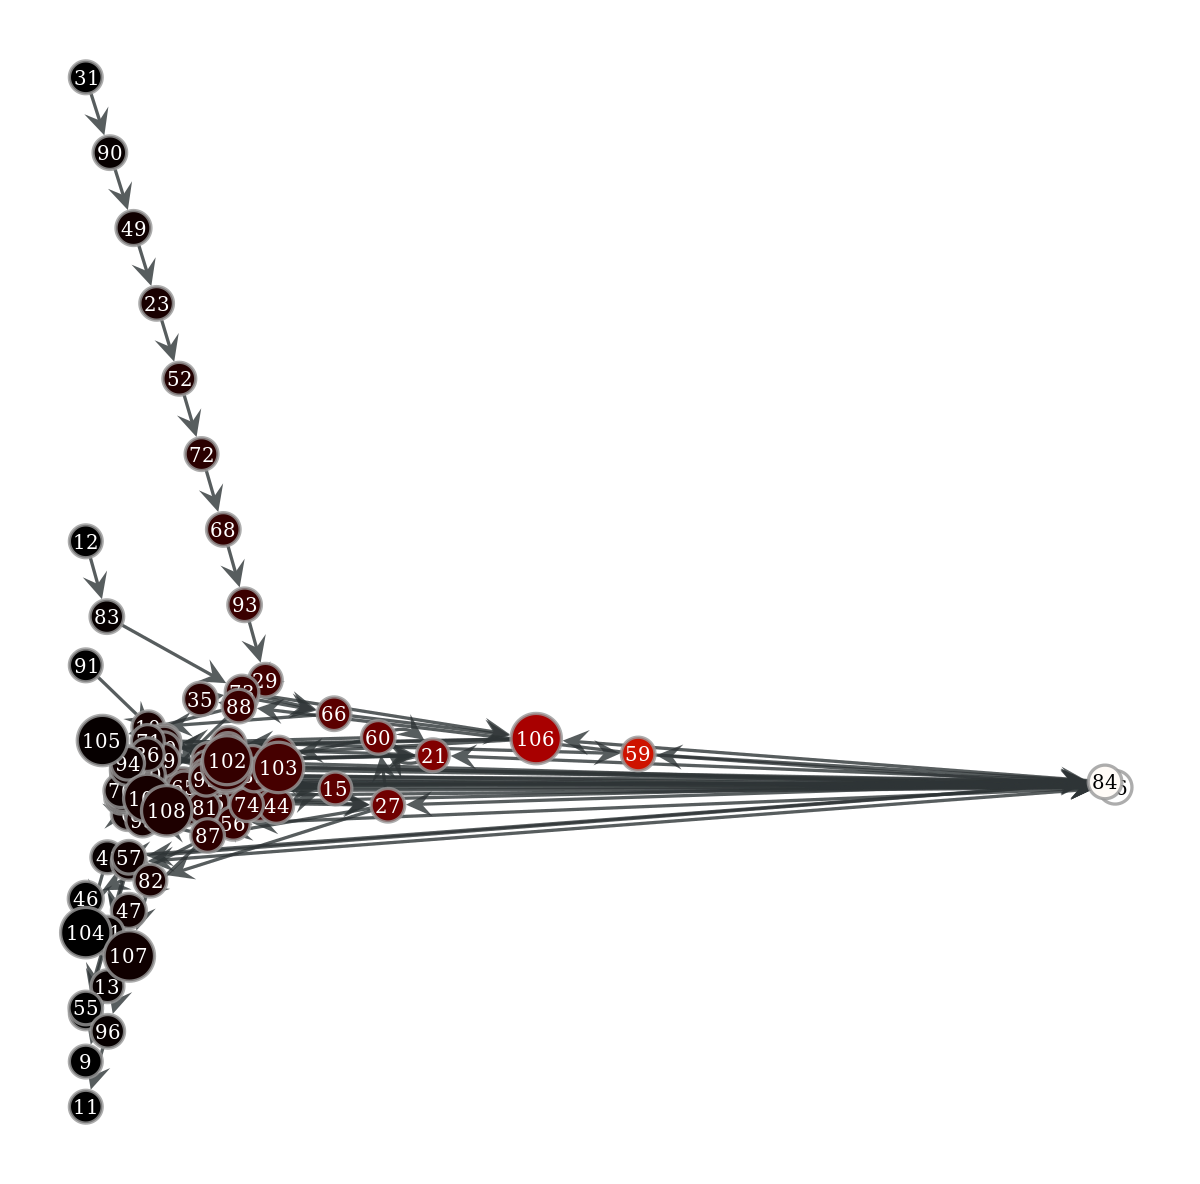
\includegraphics[scale=0.2]{germanbetweenness.png}
	\caption{Positions of the German numbered graph but with trophic levels and betweenness on the y-axis and x-axis respectively.}
	\label{fig:gerbc}
\end{subfigure}
\hfill
\begin{subfigure}{.45\textwidth}
	\hspace{-1cm} 
	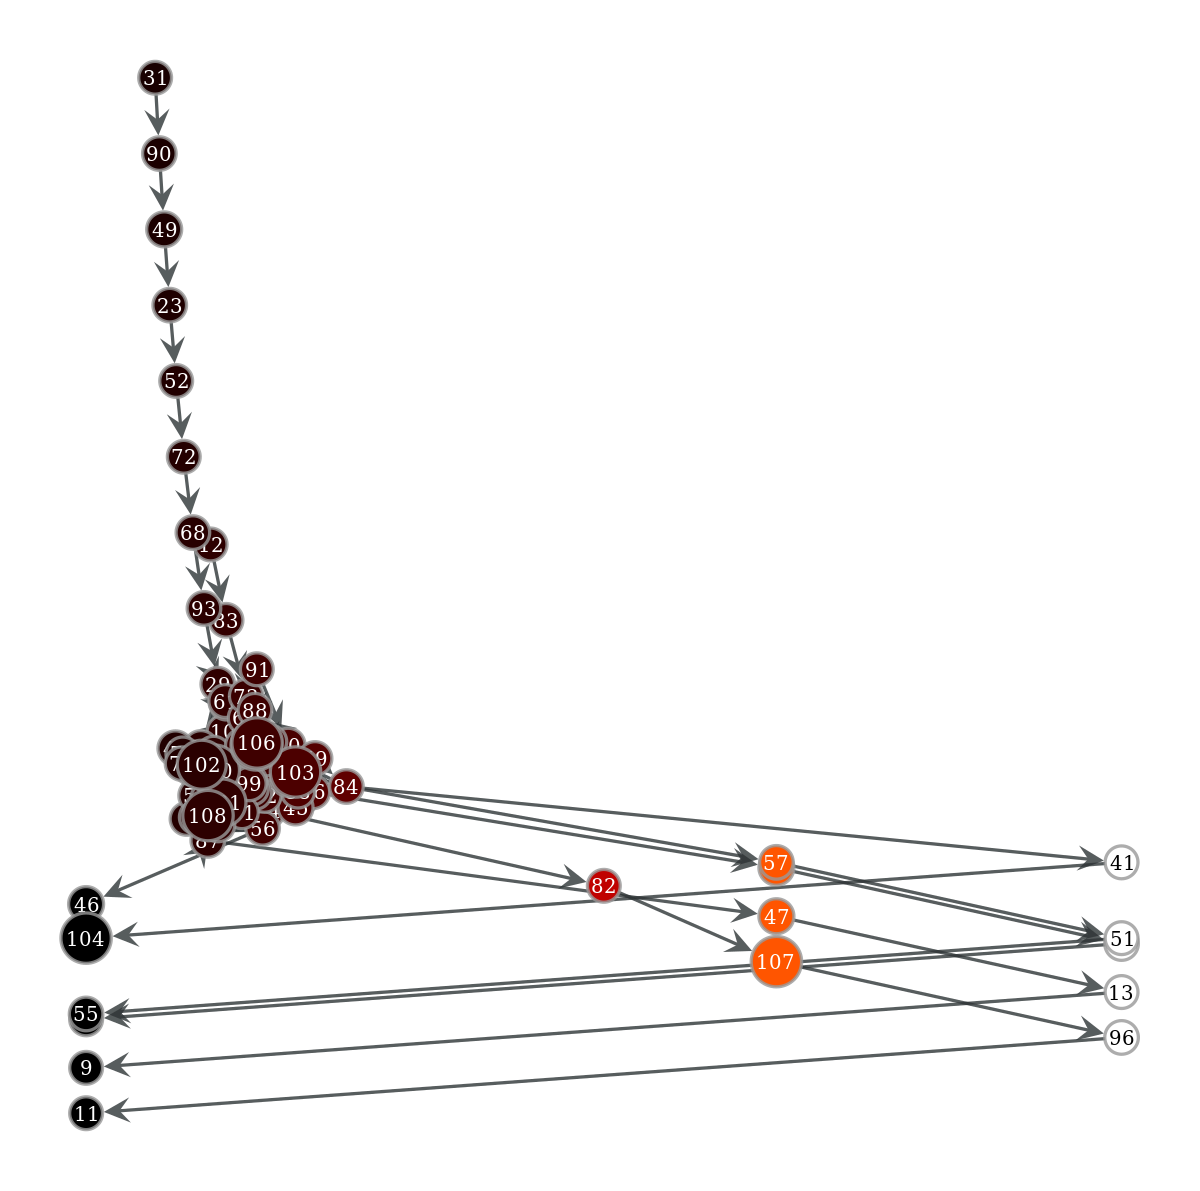
\includegraphics[scale=0.2]{germancloseness.png}
	\caption{Similar to the betweenness German graph but with closeness centrality values instead. }
	\label{fig:gercc}
\end{subfigure}
\caption{Betweenness and closeness centrality values displayed on the x-axis based on the German numbered word graph.}
\label{fig:gercentrality}
\end{figure}

Assessing the graphs visually through Figures \ref{fig:gerbc} and \ref{fig:gercc}. Vertices 84 and 26 have the highest betweenness which correlates to the the frequencies of the words in the German Story Corpus. This was also the case of the English version as these refer to the words "ein" and "und" which are the most commonly used as bridges/links in sentences.

With closeness centrality, since it is a measure of influence on nearby words, the graph shows that the vertices 97, 13, 33, 51 and 41 has the largest values. These all correlate to the second to last word of each sentence apart from the first sentence which has the word "Kind". However "Kind" is used elsewhere meaning that the vertices mentioned before are unique and essential as a bridge in it's nearby words. Otherwise the graph will be disconnected if they are removed. Note that the orange vertices in Figure \ref{fig:gercc} are the unique words predecessors to the vertices mentioned earlier and the last word of every sentence always has a value of zero.

Therefore betweenness identifies the words of key importance that are used most commonly as connectors. Meanwhile closeness identifies the words most likely to isolate vertices of the graph when following the sentence flow, i.e. breaks up the rest of the sentence into unique words.

\begin{figure}[H]
\centering
\begin{subfigure}{.45\textwidth}
	\hspace{-1cm} 
	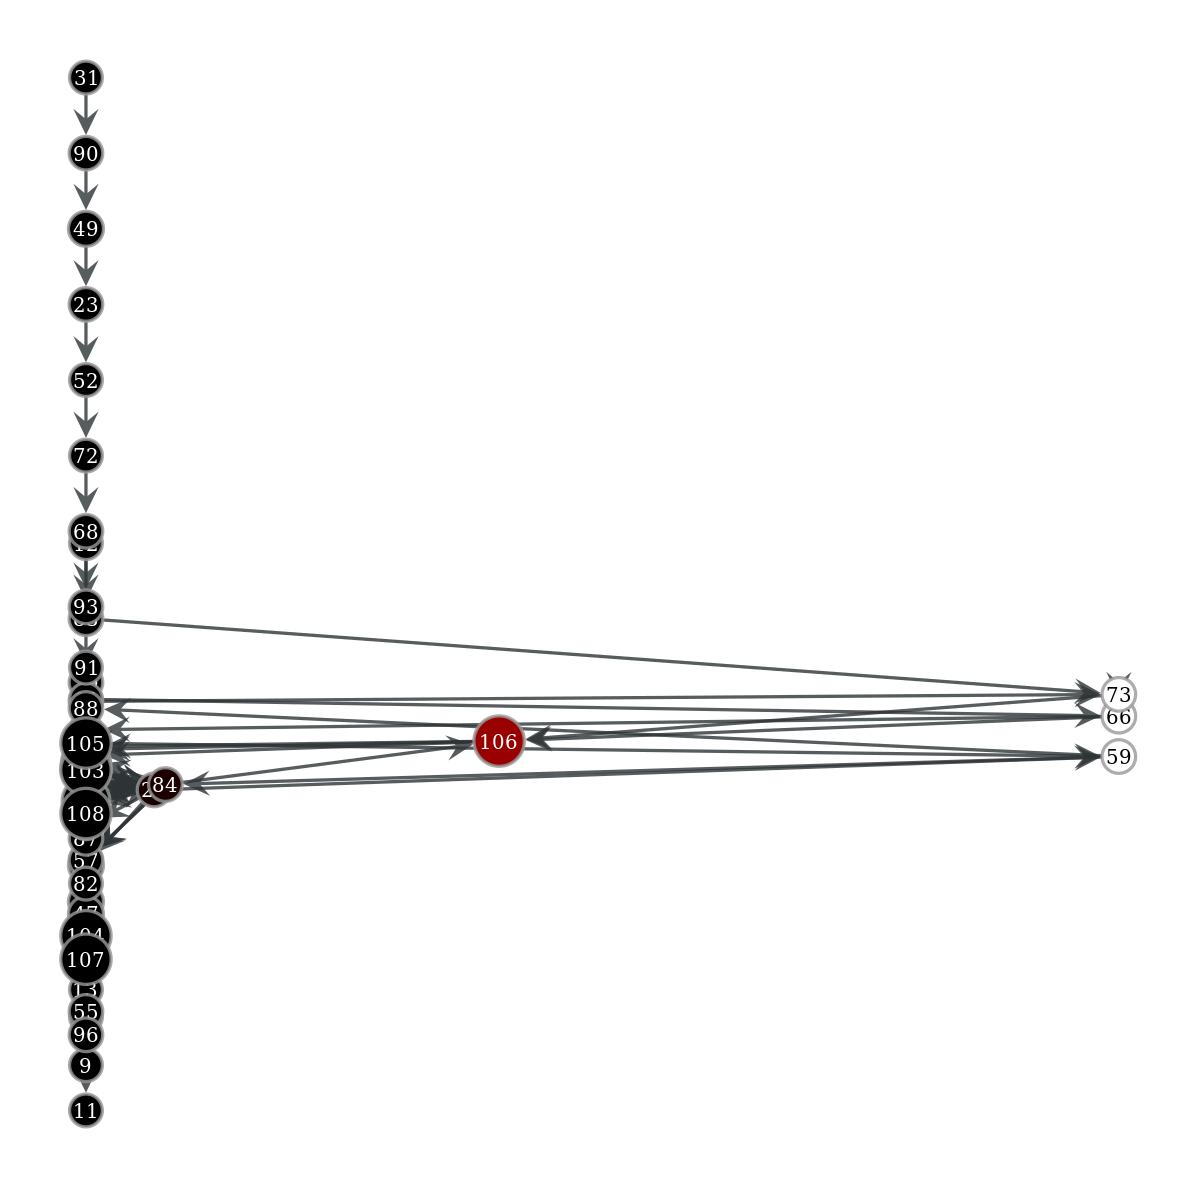
\includegraphics[scale=0.2]{germanlocalclustering.png}
	\caption{Displays the local clustering coefficient against the trophic levels.}
	\label{fig:gerlc}
\end{subfigure}
\hfill
\begin{subfigure}{.45\textwidth}
	\hspace{-1cm} 
	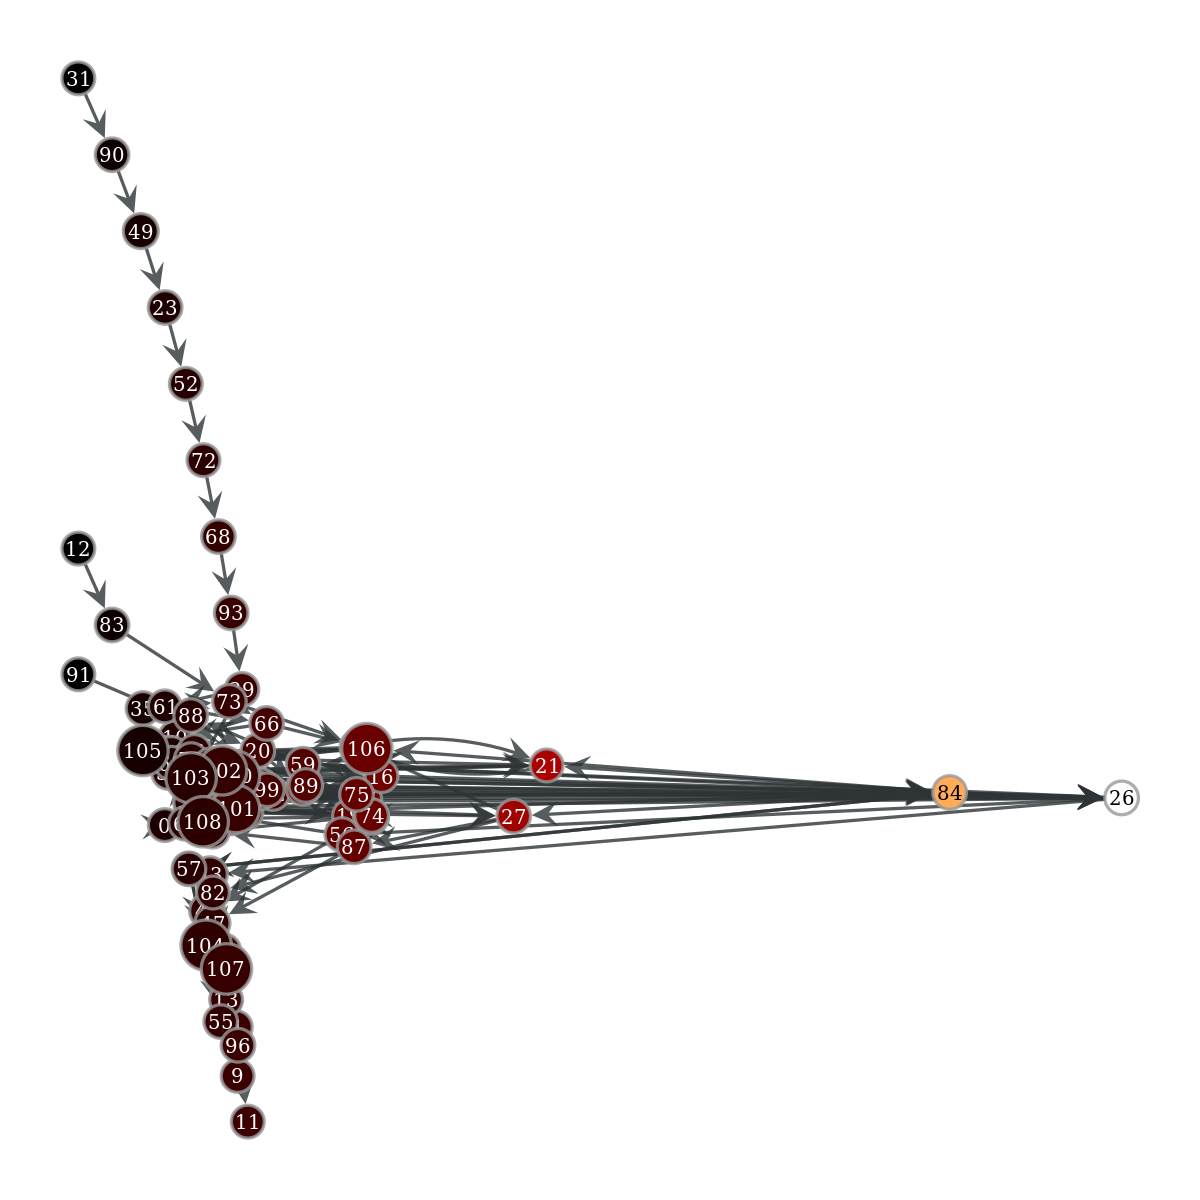
\includegraphics[scale=0.2]{germanpagerank.png}
	\caption{Displays the page rank against the trophic levels.}
	\label{fig:gerpr}
\end{subfigure}
\caption{Displays the local clustering and page rank on the x-axis instead of the centrality values.}
\label{fig:gerother}
\end{figure}

Nothing clear can be correlated by studying the local clustering as almost all have a local clustering of zero apart from six vertices. Three of which are vertices 57, 73 and 66 which corresponds to the words "könig", "sich" and "nicht" which are not unique words in the German story corpus. Whereas vertices with a high page rank correlate to either conjunctions, vertex 84 (und), or words that accompany other words like pronouns or articles, vertices 26 (ein), 27 (eine) etc. Therefore high page rank relates to basic building blocks for the language that are used frequently frequently, can be extended to the German language as a whole.

In conclusion, similar results were seen when analysing the graphical properties based on the German and English translations. With German having a clearer visualisation and stronger correlation compared to the English language due to having inflections.


\section{Japonic}
Moving to a different language family. The Japonic language family is the protolanguage for Japanese and Ryūkyūan languages\cite{vovin2017origins} so it is a small language family compared to other language families like the Indo-European family. Translating the corpus into Japanese gives us a new dataset to use for graph property analysis which will be studied in comparison to the previous language family. Japanese translation of the story will be referred to as the Japanese corpus and the same 
\subsection{Japanese}
To give a larger variety of languages, Japanese is studied as it uses vastly different grammar compared to other languages. Japanese has only five lexical word classes which includes nouns, verbal nouns, nominal adjectives, verbs and adjectives. The order in which the words are structured are different to Indo-European languages since Japanese uses SOV (Subject-object-verb) compared to languages like German and English which uses SVO (Subject-verb-object). As well as this, Japanese does not have major reliability on grammatical number or gender and is more focused on their system of honorifics which indicates the speaker, listener or person it references. Therefore, Japanese may have words borrowed from other languages (these are reffered to as loanwords\cite{miura1979influence}) but their grammar is different in comparison. 

We follow the same process as before and input the Japanese Story corpus into my program to produce the basic graphs. For simplicity, we just show the numbered version of the word graph (see Figure \ref{fig:jpgraph}) with the words they reference to in the table of data (See Table ??).

\begin{figure}[H]
\centering
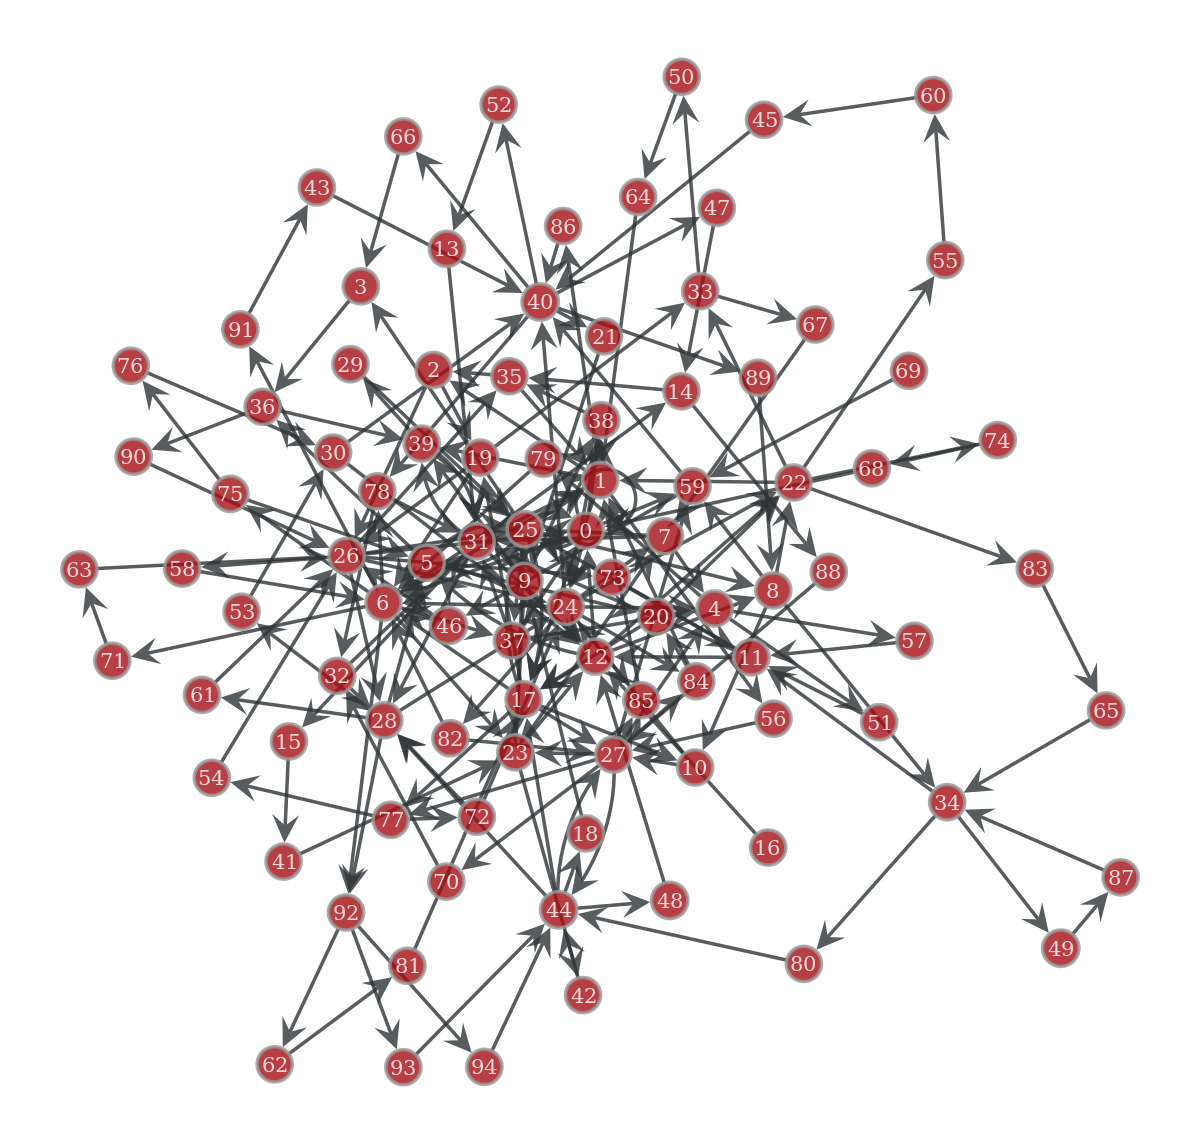
\includegraphics[scale=0.25]{japanesewordgraph.png}
\caption{The Japanese word graph and numbered equivalent of the word graph generated from the Japanese translation of the "Sleeping Beauty" corpus.}
\label{fig:jpgraph}
\end{figure}

With previous languages having a largest frequency of nine, with Japanese there are six words with eleven or more appearances (see Table \ref{table:japanesetop}), largest being fourteen for vertex 17. This word is a form of conjugation which means that it's use depends on the inflections of it's associated words. Generally vertex 17 is most commonly used to express the past tense for the phrase in context. So rather than having a separate word for different tenses, Japanese uses accompanying words instead which leads to the higher frequency counts for said words. Furthermore, this is the case for most of the word with a large count like how vertex 12 is used to empathically add more information (an empathic and), vertex 6 is a particle so means "but" or indicated the sentence subject. Therefore, Japanese words has heavy reliability on each other to define their meaning so the graph contains a lot of edges denoting these relationships. We study other properties to see if there is other correlation.

\begin{table}[H]
\centering
\begin{subtable}{.45\textwidth}
	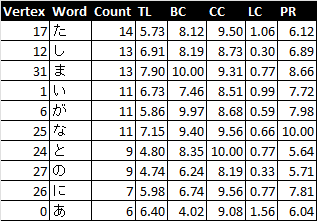
\includegraphics[scale=0.9]{japanesetabletop10.png}
	\caption{Top 10 words with the highest frequency in the German translation of the corpus. Shown in table format with other graphical properties. }
	\label{table:japanesetop}
\end{subtable}
\hfill
\begin{subtable}{.45\textwidth}
	\hspace{1.5cm} 
	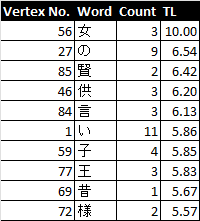
\includegraphics[scale=1]{jptabletc.png}
	\caption{Top 10 works with highest trophic levels in the German translation dataset.}
	\label{table:japanesentoptc}
\end{subtable}
\caption{Partial extracts of the table data for graphical properties of the German Story Corpus.}
\end{table}

Trophic levels cannot be applied to this dataset like with previous languages. This is due to the graph having bidirectional edges such as the edge between vertex 25 and 5 which is part of the sentence about having only 12 plates. Also vertex 0 contains a self loop which and is part of the word "everyday". So there is not a clear hierarchical structure to be inferred to. The largest trophic level is vertex 56 (refers to female) which appears in middle of sentences with the Japanese story corpus. Currently the trophic levels cannot be calculated accurately but can be if the dataset is split into specific group of words depending on it's meaning rather than character by character. For example vertex 59 and 46 means "child" together but is split in the dataset as the program doesn't recognise characters together as a singular word. However this either requires the full understanding of the Japanese language or heavy cross-referencing and checking. 

\begin{figure}[H]
\centering
\begin{subfigure}{.45\textwidth}
	\hspace{-1cm} 
	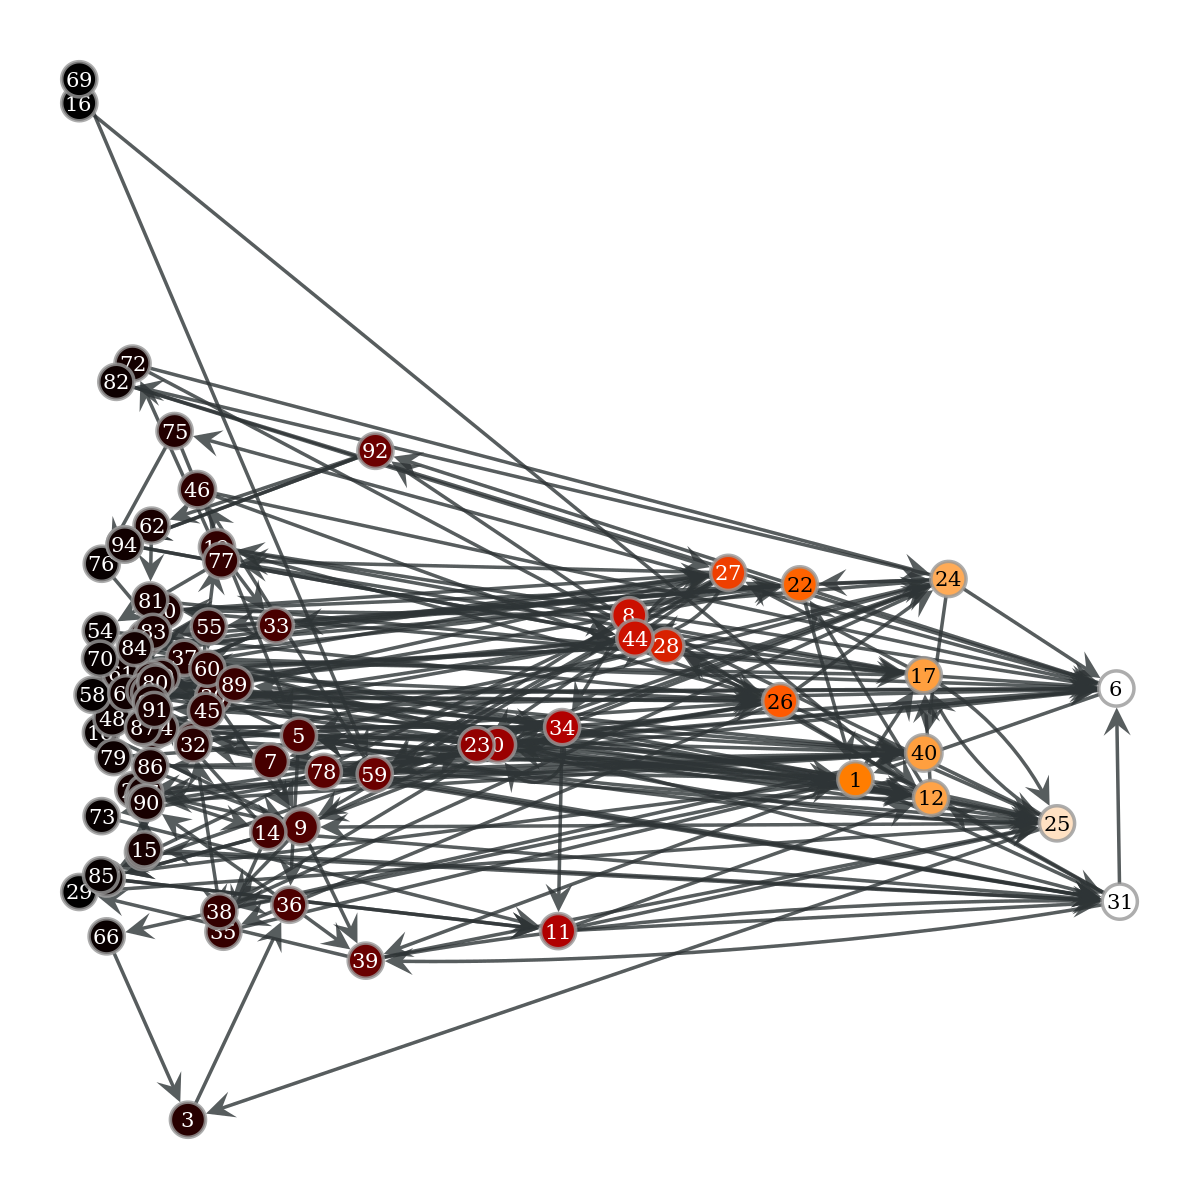
\includegraphics[scale=0.2]{japanesebetweenness.png}
	\caption{Positions of the German numbered graph but with trophic levels and betweenness on the y-axis and x-axis respectively.}
	\label{fig:jpbc}
\end{subfigure}
\hfill
\begin{subfigure}{.45\textwidth}
	\hspace{-1cm} 
	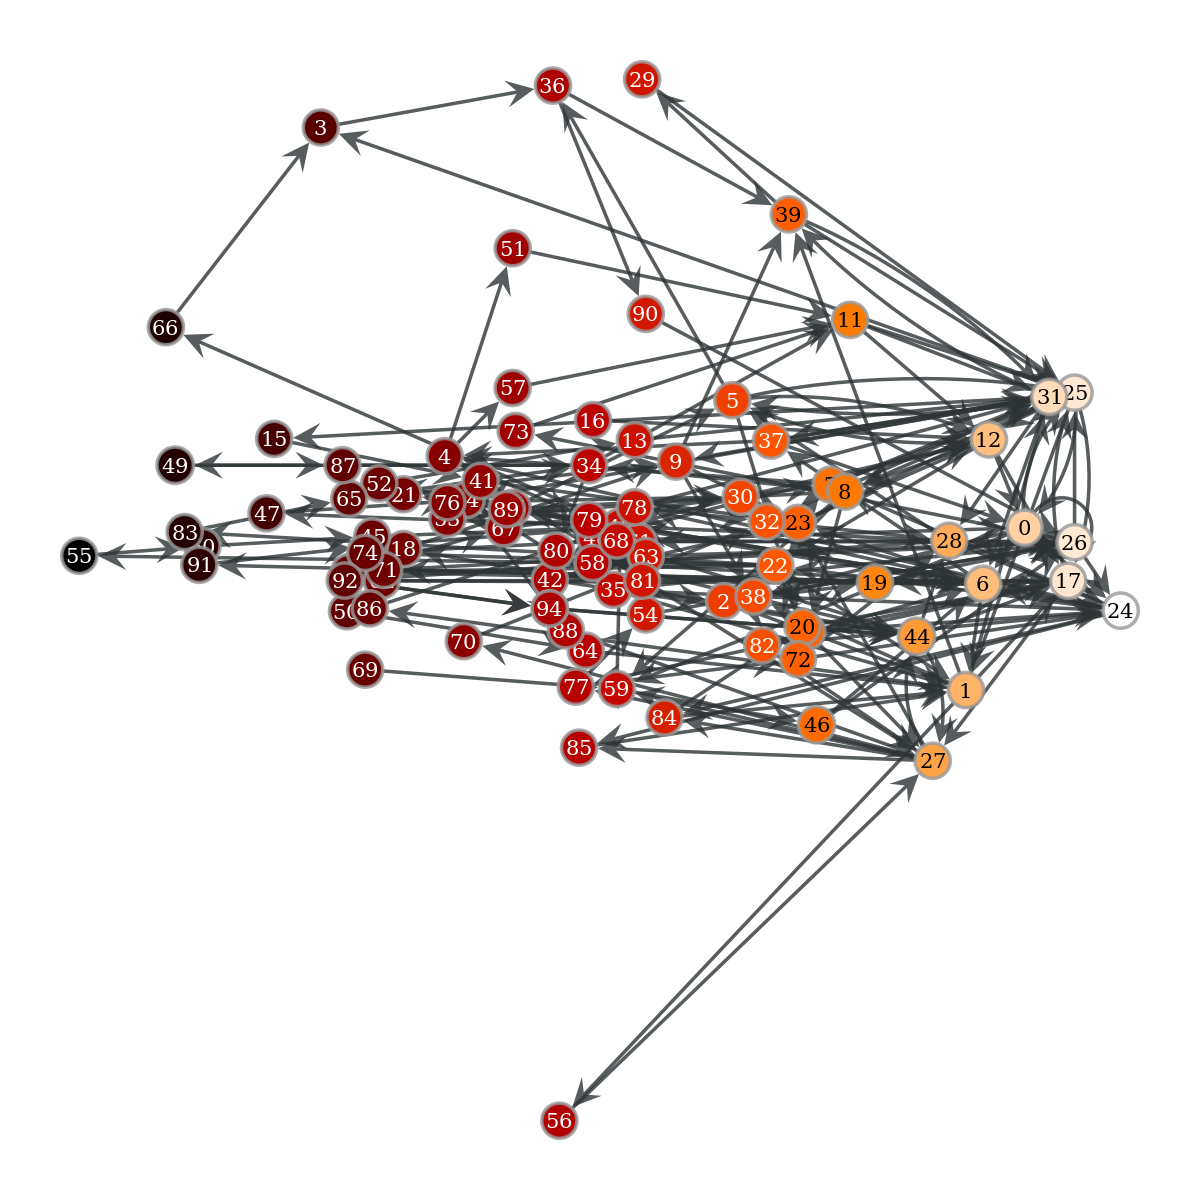
\includegraphics[scale=0.2]{japanesecloseness.png}
	\caption{Similar to the betweenness German graph but with closeness centrality values instead. }
	\label{fig:jpcc}
\end{subfigure}
\caption{Betweenness and closeness centrality values displayed on the x-axis based on the German numbered word graph.}
\label{fig:jpcentrality}
\end{figure}

The graphs in the centrality figure \ref{fig:jpcentrality} shows that the words are more evenly distributed unlike the Indo-European languages. Which correlates to the importance of the Japanese characters nature of being reliant on one another for their meaning and demonstrates the complexities of the language. However higher betweenness still correlates to the character's importance within the corpus where other characters require them to complete their meaning or structure. Although further detailed cannot be determined by the visualisation other than importance.

Japanese's closeness centrality values has a larger average than Indo-European languages. The closeness is a closer look on the betweenness centrality so all vertices in the betweenness graph is essentially shifted right if the vertices have connections to the vertices of high betweenness.

Therefore only a general correlation can be demonstrated through the centrality graphs. Clearly results can be gathered with a better reword or Japanese fluency.

\begin{figure}[H]
\centering
\begin{subfigure}{.45\textwidth}
	\hspace{-1cm} 
	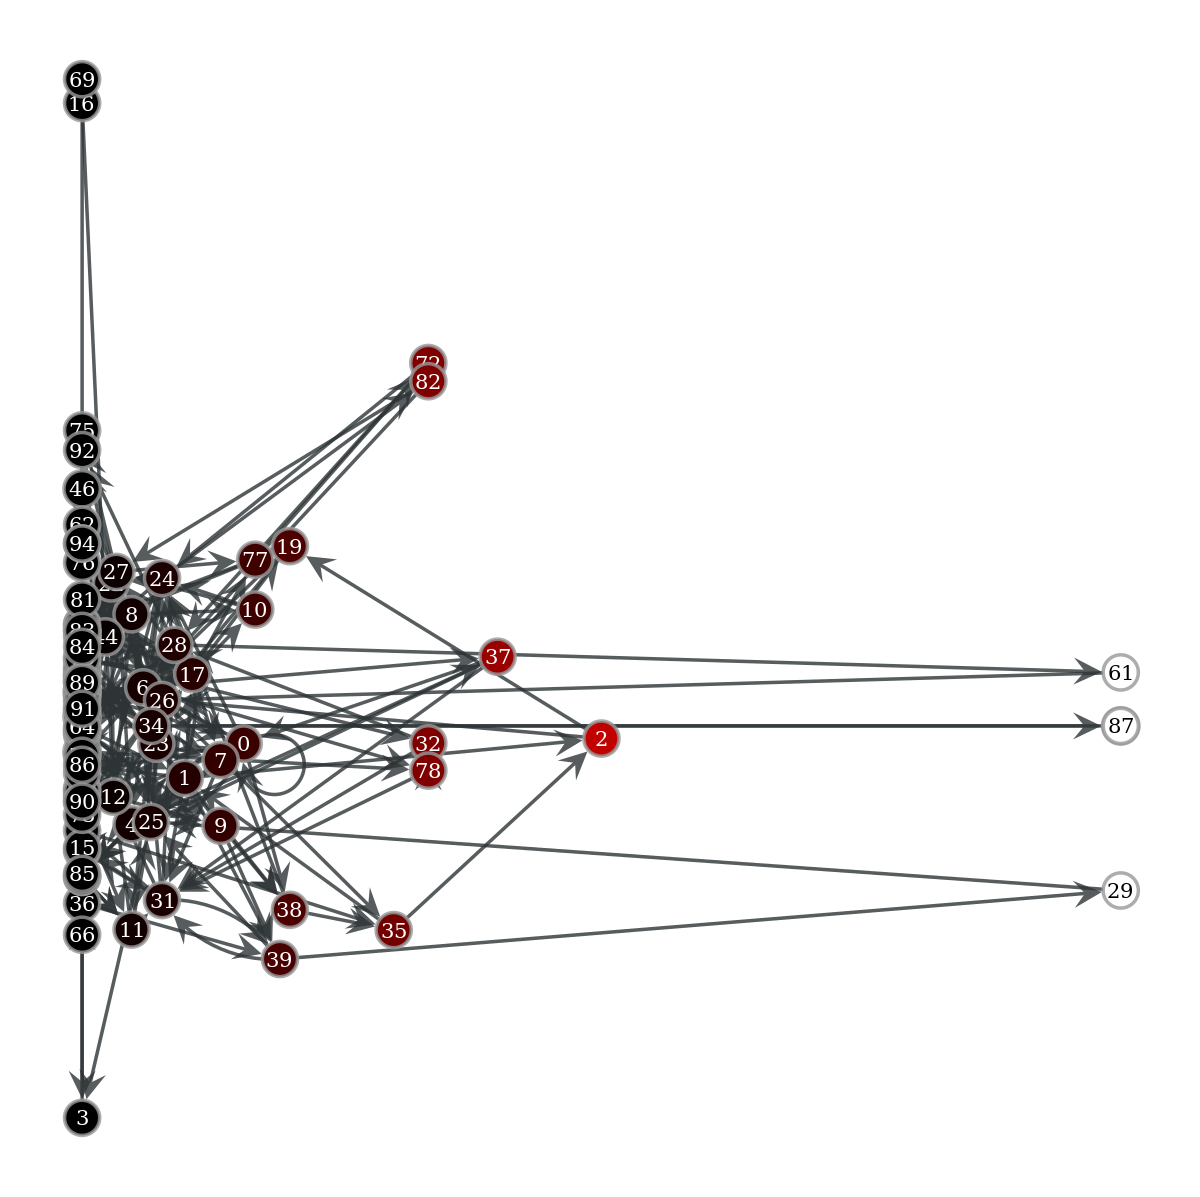
\includegraphics[scale=0.2]{japaneselocalclustering.png}
	\caption{Displays the local clustering coefficient against the trophic levels.}
	\label{fig:jplc}
\end{subfigure}
\hfill
\begin{subfigure}{.45\textwidth}
	\hspace{-1cm} 
	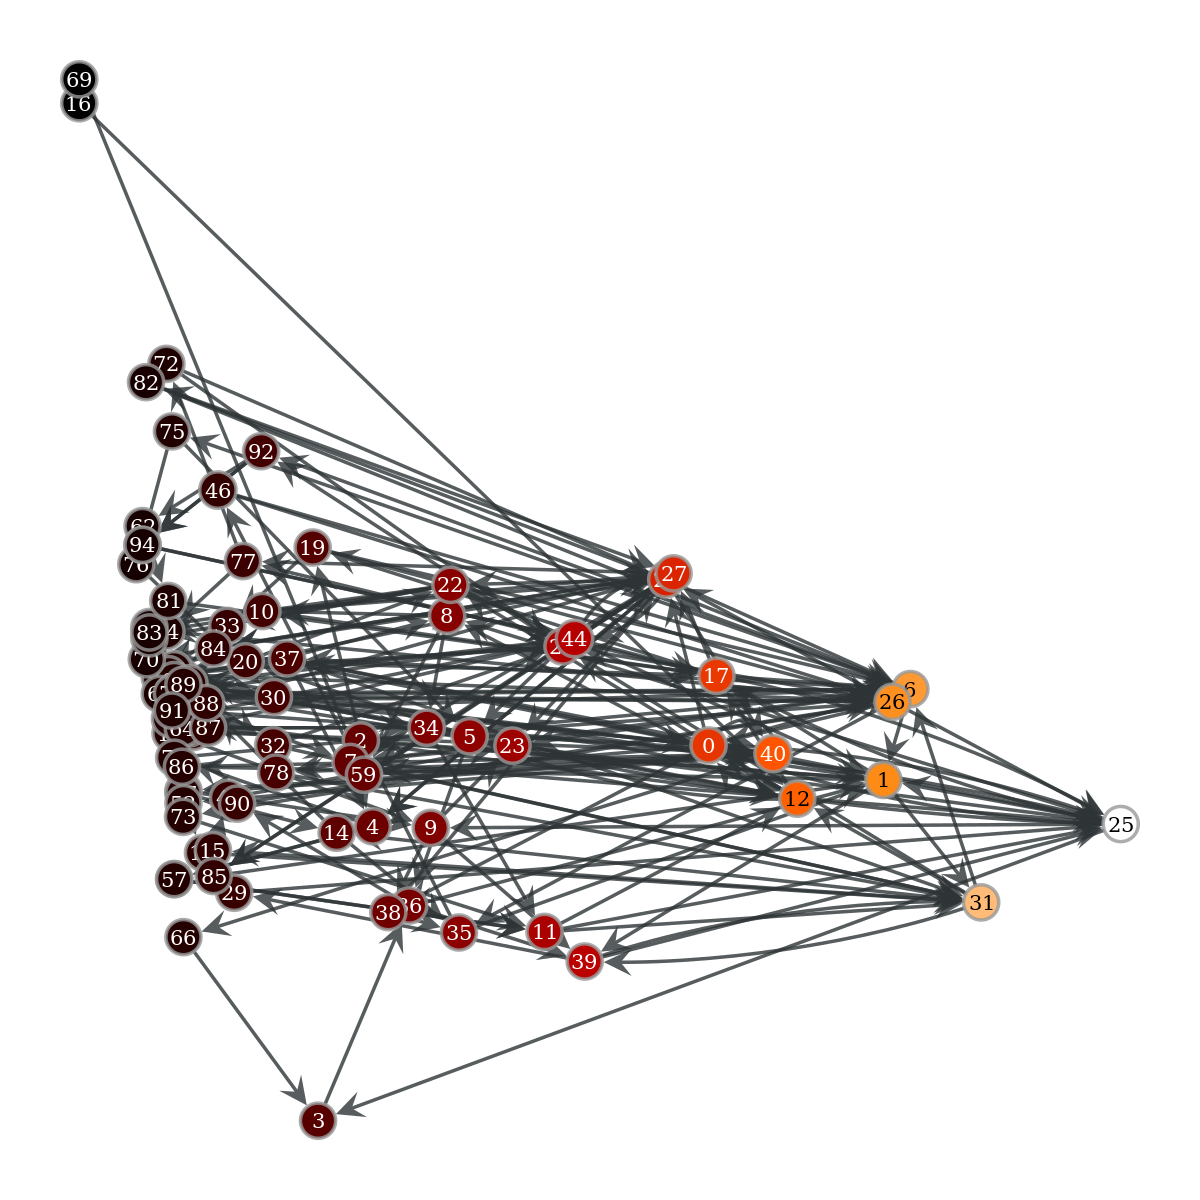
\includegraphics[scale=0.2]{japanesepagerank.png}
	\caption{Displays the page rank against the trophic levels.}
	\label{fig:jppr}
\end{subfigure}
\caption{Displays the local clustering and page rank on the x-axis instead of the centrality values.}
\label{fig:jpother}
\end{figure}

Local clustering (see the graph in Figure \ref{fig:jplc}) measures how close the vertex is part of a unique directed triangle, i.e. a directed 3 cycle. The vertices 29, 87 and 61 are vertices who are involved in such triangles where they each have a unique in and out edge to other vertices. Lower values means they are not involved in many triangles. Thus local clustering can identify certain triples in the Japanese texts that would have unique meanings. 

Page rank derives the vertices who have an influence to other vertices nearby but not immediate neighbours like what closeness does. However nothing further can be correlated based on this graph (see Figure \ref{fig:jppr}).

In conclusion the way the Japanese story corpus is split into the database (character by character), only general correction can be determined based upon the graphs and their properties. Stronger links as to what exact words have importance cannot be obtained here without the full understanding of the language. On the other hand, we see that in general the graphs are different to the ones based on the Indo-European languages which demonstrates their differences. To see this further we analyse another language and it's language family.

\section{Sino-Tibetan}
This is the final language family we analyse. 


\subsection{Chinese}

